\documentclass[a4paper, 11pt]{article}

\usepackage[utf8]{inputenc}
\usepackage{a4wide}
\usepackage{indentfirst}
\usepackage{hyperref}
\usepackage{url}
\usepackage{graphicx}
\usepackage{float}
\usepackage{relsize}
\usepackage{setspace}

\onehalfspacing

\title{CVE-2017-5638 \\ [0.8em] \smaller Apache Struts Vulnerability}
\author{}
\date{}

\begin{document}

\maketitle

For this presentation, we chose to analyze a vulnerability related to Apache Struts, which is described
in the CVE-2017-5638.

\section{Context}

Apache Struts is a free, open-source, MVC framework for creating modern Java web applications. Basically,
the Jakarta Multipart parser in Apache Struts 2 mishandles file upload, which allows remote attackers
to execute arbitrary commands. 

We will now give a more in depth explanation of this vulnerability, its impacts and countermeasures that
can be taken to reduce its consequences.

\section{Theory behind the exploit}

Struts is vulnerable to \textbf{remote command injection attacks} through the incorrect parsing of an
attacker's invalid \texttt{Content-Type} HTTP header. This vulnerability allows these commands to be
executed under the privileges of the Web server. This is full remote command execution and has been
actively exploited in the wild from the initial disclosure in March 2017.

The vulnerable code is in the Jakarta Multipart parser. If the \texttt{Content-Type} value isn't valid,
that is, if it does not match an expected valid type, an exception is thrown that is then used to display
an error message to the user.

The vulnerability occurs because the \texttt{Content-Type} is not escaped after the error, and is then used
by the function \texttt{LocalizedTextUtil.findText} to build the error message, which interprets the supplied
message. Anything within \texttt{\$\{…\}} will be treated as an Object Graph Navigation Language (OGNL)
expression and evaluated as such. This is an open-source Expression Language for Java, which allows
getting and setting properties and execution of methods of Java classes. 

The attacker can leverage these conditions to execute this kind of expressions that, in turn, can execute
system commands through \texttt{java.core.ProcessBuilder()}. Exploitation is further facilitated by the
ability to receive information back from the server on the status and output of the commands that are
executed by the web server.

\section{Exploit}

To carry out the exploitation of this vulnerability, we used a Python script which contains two important
functions. The first, \texttt{check}, checks if a given web site is vulnerable to this attack. The other
function, \texttt{exploit}, enables us to carry out the exploit and execute a given command of our choosing.

\subsection{Function check(url)}

As we can see in this snippet, an OGNL expression in injected into the payload of a request in order
to add a parameter to the response headers.

We can determine weather a certain web application is vulnerable to this attack by determining if the
response headers includes the parameters we previously tried to add.

\vspace{2cm}

\begin{figure}[H]
    \centering
    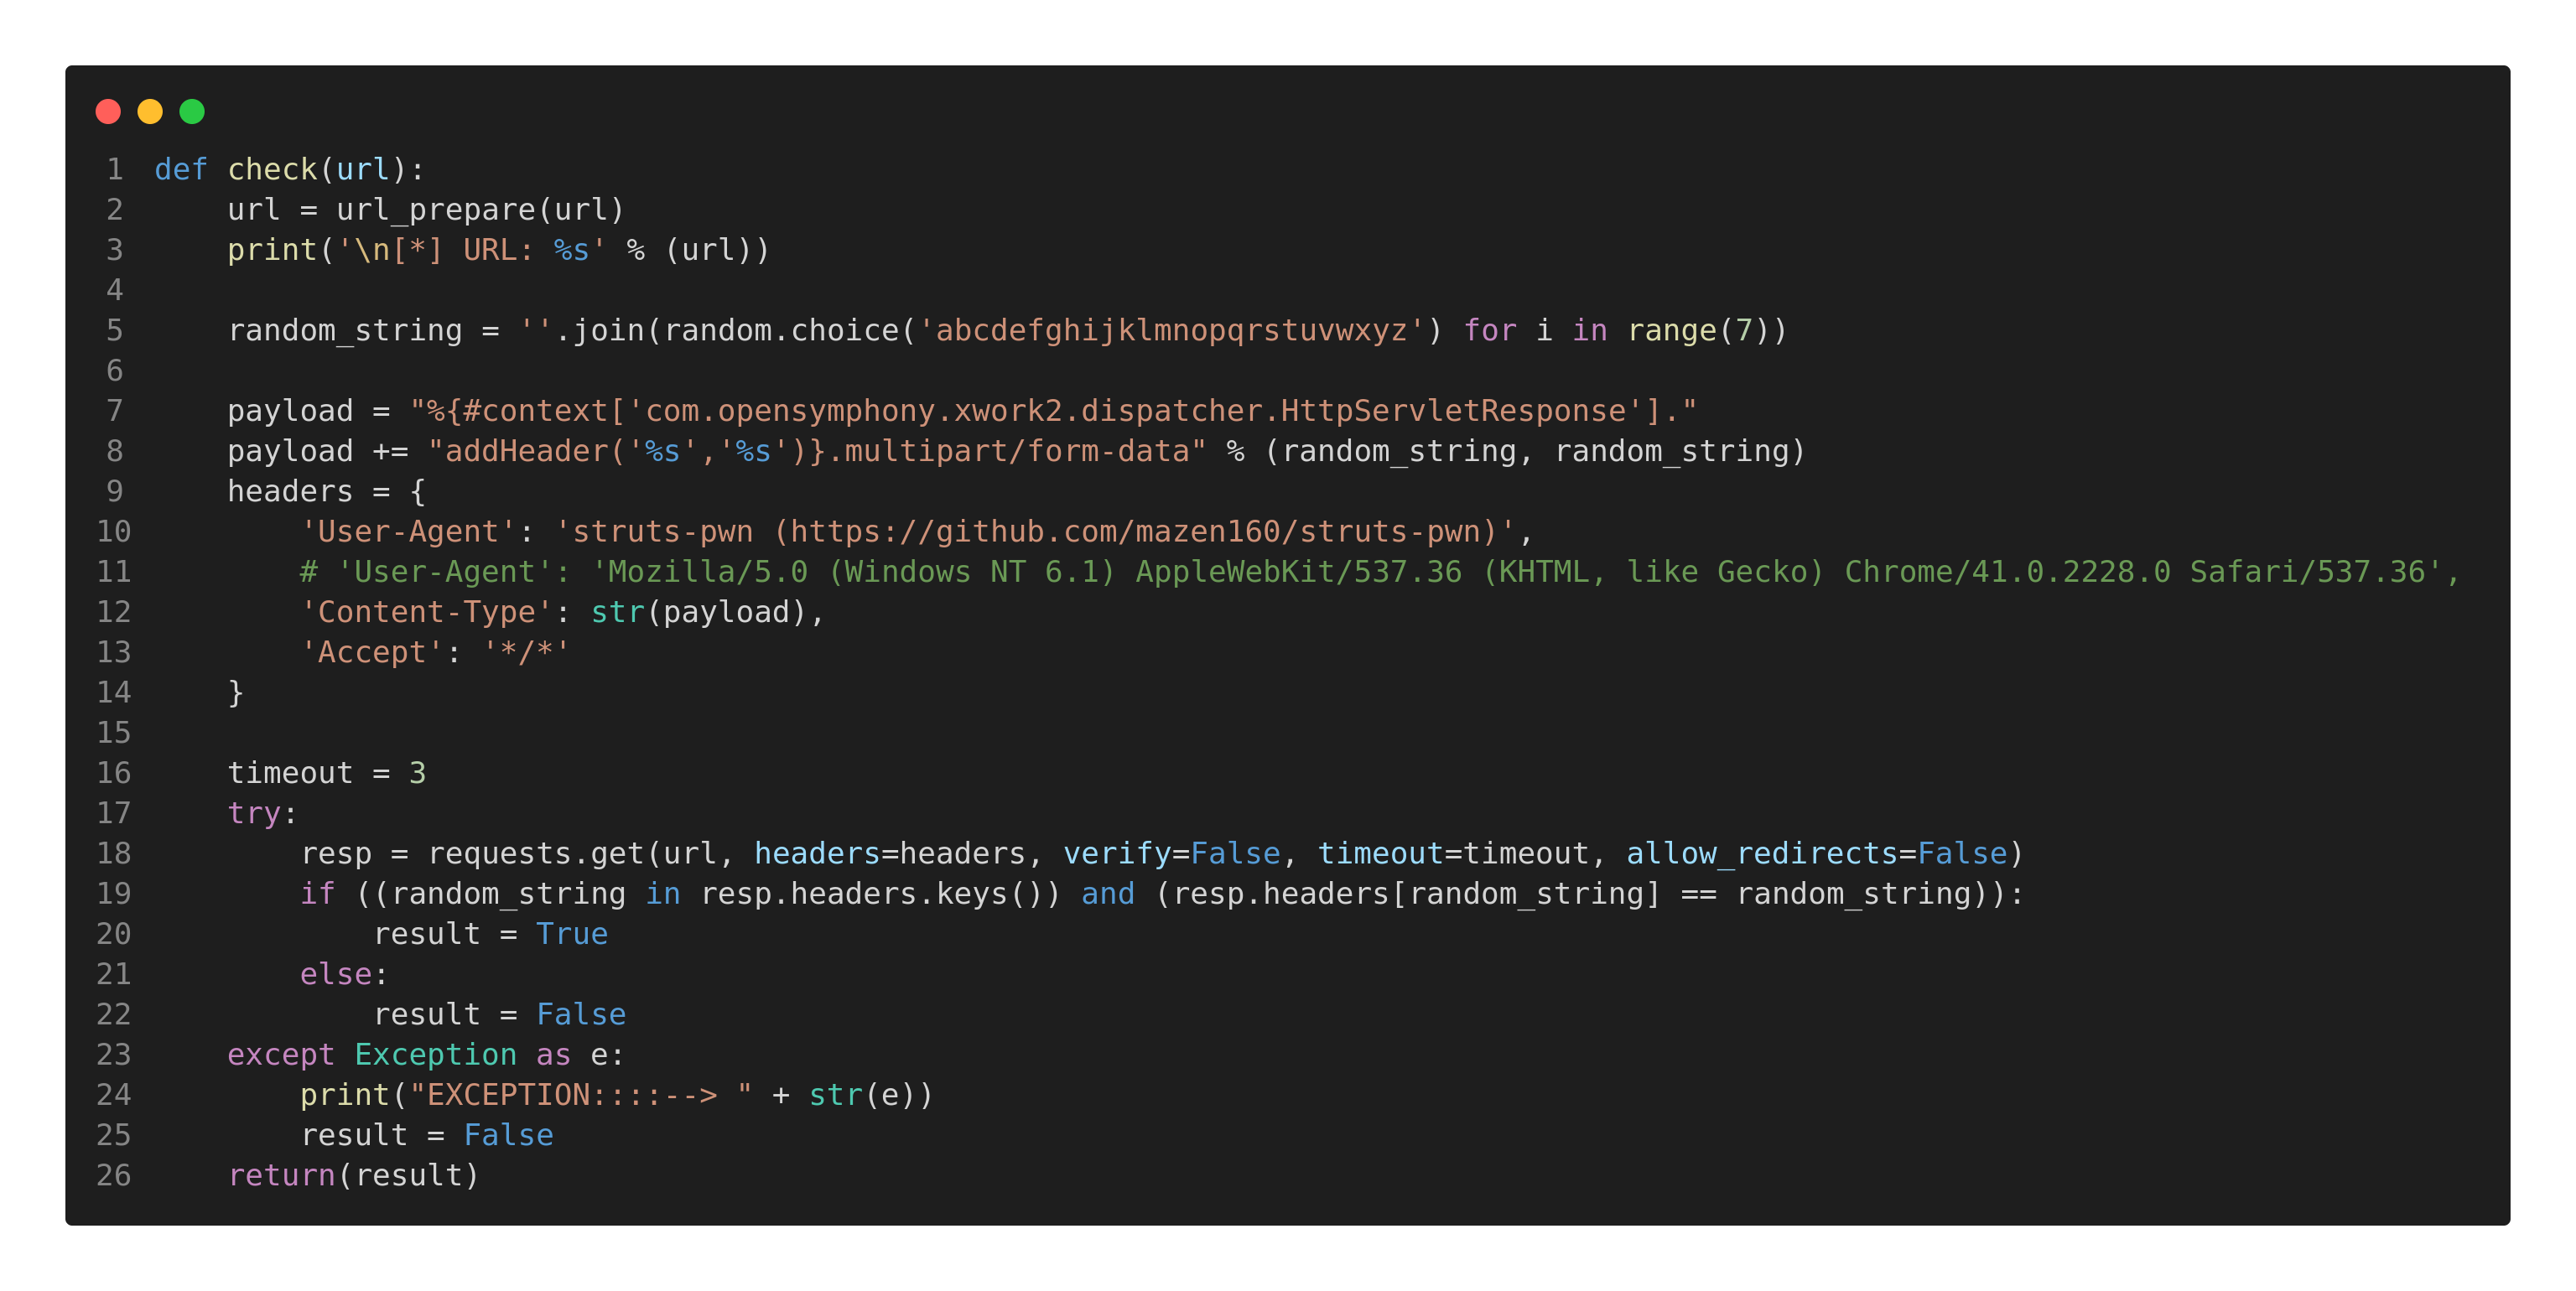
\includegraphics[width=\textwidth]{img/check.png}
\end{figure}

\pagebreak

\subsection{Function exploit(url, cmd)}

After determining if a web application is vulnerable to this attack, we can carry out the exploitation
itself. To do so, the function \texttt{exploit} injects the specified command in the payload of a request.
This command will then be executed by the web server and the output will be sent to the attacker in the
response.

\begin{figure}[H]
    \centering
    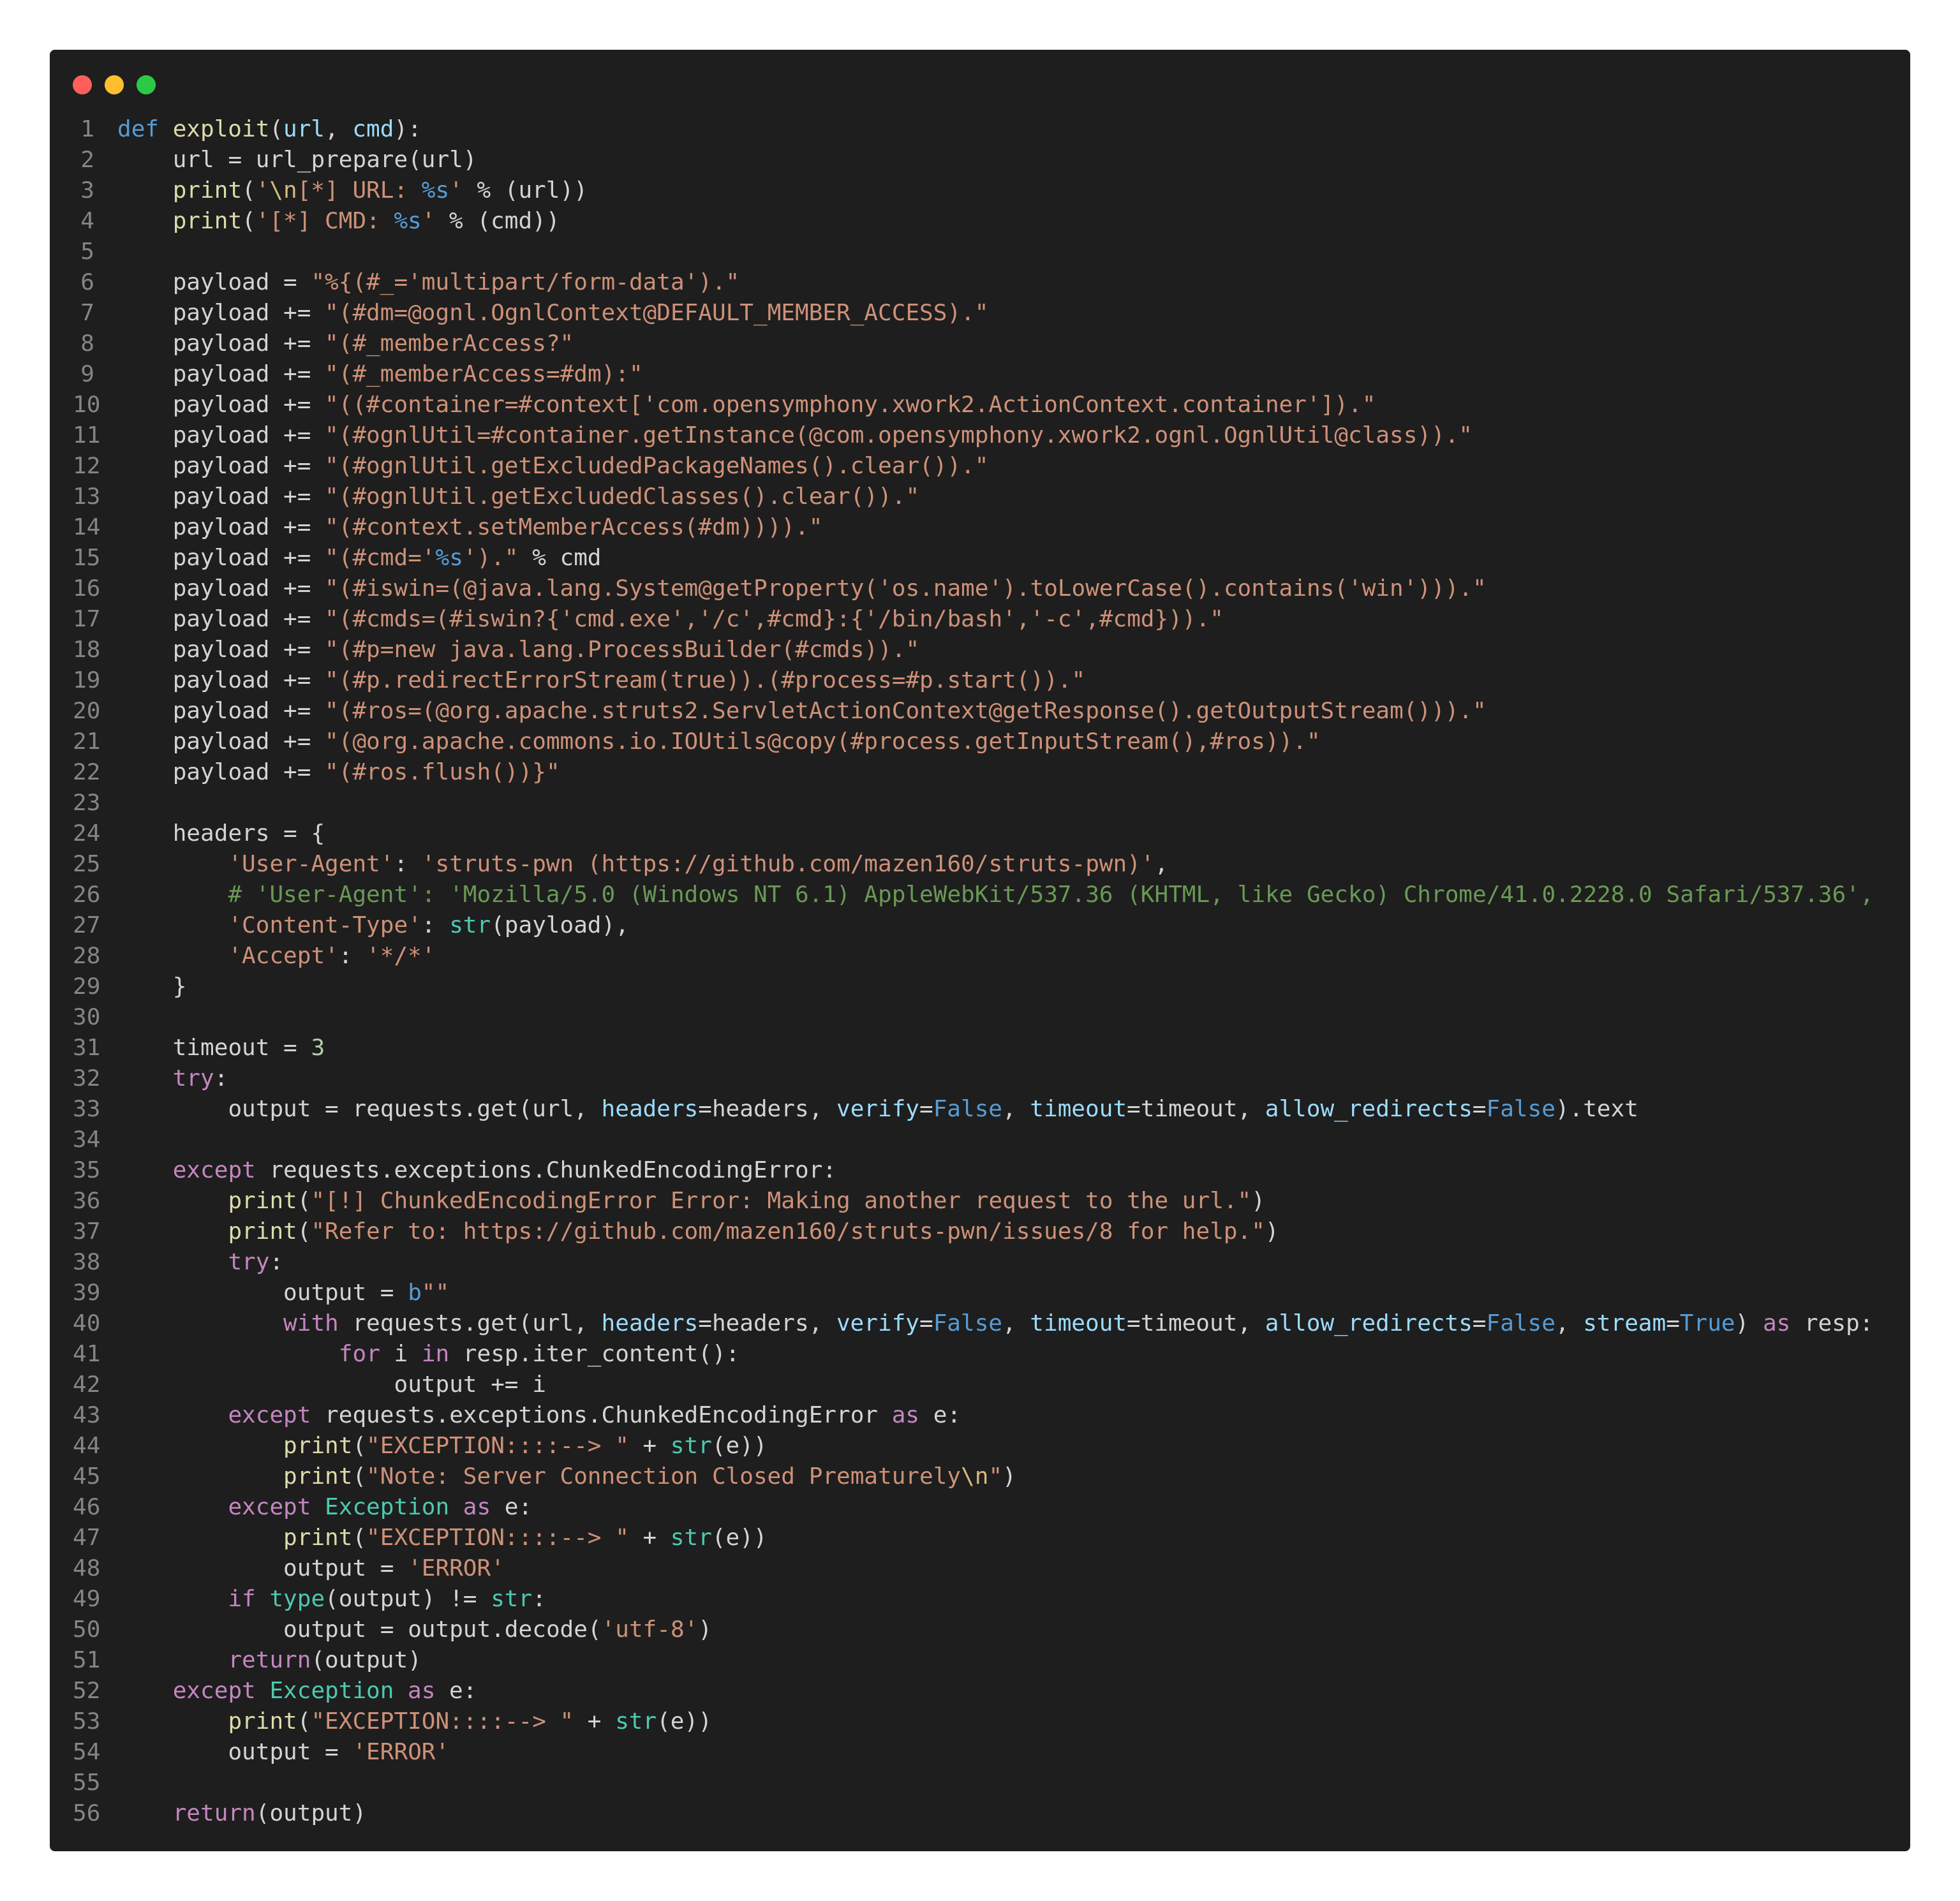
\includegraphics[width=\textwidth]{img/exploit.png}
\end{figure}

\pagebreak

\section{Impact}

This vulnerability allows a remote attacker to inject operating system commands into a web application
through the \texttt{Content-Type} header.

In fact, it makes remote code execution (RCE) possible, which enables the attacker to run code of their
choosing with system level privileges on the server.

Once sufficiently compromised, the attacker may be able to access any information on a server such as
databases containing sensitive information.

What makes this particularly dangerous is not only the real threat of information theft and other risks
associated with running arbitrary code on the server, but the difficulty in detecting this defect.

It is also worth noting that since Struts is widely used, non-targeted attacks are also likely to occur.

\section{Countermeasures}

Web application firewalls could mitigate this attack if the rules are set to approve valid content
types or ban OGNL expressions.

However, a simpler approach such as upgrading to Apache Struts version 2.3.32 or 2.5.10.1., which are
not vulnerable to this attack, is enough.

Finally, one could switch to a different implementation of the Multipart parser such as the Jason Pell’s
Multipart parser.

\section{Demo}

We're now going to perform a live demonstration of this vulnerability.

First, we have to pull a docker image with a vulnerable version of the Apache Struts2.

\begin{verbatim}
$ sudo docker run -p8080:8080 -ti piesecurity/apache-struts2-cve-2017-5638
\end{verbatim}

After starting the container, the web app is now visible on port \texttt{8080}.

\begin{verbatim}
$ firefox "http://localhost:8080/fileupload.action" &
\end{verbatim}

Then, we download a Python script that has the utility functions we mentioned previously so we can
check and exploit this vulnerability.

\begin{verbatim}
$ git clone https://github.com/mazen160/struts-pwn.git && cd struts-pwn
$ ./struts-pwn.py --check --url 'http://localhost:8080/fileupload.action'
\end{verbatim}

As we can see, this endpoint is vulnerable.

\pagebreak

We can now execute some commands to the server with the flag \texttt{-c}.

\begin{verbatim}
$ ./struts-pwn.py --url 'http://localhost:8080/fileupload.action' -c 'whoami'
\end{verbatim}

As we can see, we just printed the user responsible for running the web server. Similarly, we can run
any command we want. On the other hand, checking this logs, we can see that the web server is throwing
exceptions with invalid formats.

\end{document}
